%!TEX program = pdflatex
% Full chain: pdflatex -> bibtex -> pdflatex -> pdflatex
\documentclass[11pt,en,cite=authoryear]{elegantpaper}

\title{ElegantPaper: An Elegant \LaTeX{} Template for Working Papers}
\author{Ethan DENG \\ Fudan University \and Dongsheng DENG \\ PA Technology}
\institute{\href{https://github.com/ElegantLaTeX}{Elegant\LaTeX{} Program}}

\version{0.09}
\date{\today}

% cmd for this doc
\usepackage{array}
\newcommand{\ccr}[1]{\makecell{{\color{#1}\rule{1cm}{1cm}}}}

\begin{document}

\maketitle

\begin{abstract}
This documentation illustrates the usage of the \href{https://github.com/ElegantLaTeX/ElegantPaper}{ElegantPaper} template. This template is based on the standard \LaTeX{} article class, which is designed for working paper writing. With this template, you can get rid of all the worries about the format and merely focus on writing. For any question, please leave a message on \href{https://github.com/ElegantLaTeX/ElegantPaper/issues}{GitHub::ElegantPaper/issues}. Want to know more about Elegant\LaTeX{} Templates? Please visit: \href{https://github.com/ElegantLaTeX}{https://github.com/ElegantLaTeX}.\par
\keywords{Elegant\LaTeX{}, Working Paper, Template}
\end{abstract}


\section{Introduction}

This template is based on the standard \LaTeX{} article class, hence the arguments of article class are acceptable (\lstinline{a4paper}, \lstinline{10pt} and etc.). Alternative engines are \hologo{pdfLaTeX} and \hologo{XeLaTeX}.

\begin{lstlisting}
\documentclass[a4paper,11pt]{elegantpaper}
\end{lstlisting}
\textbf{Note:} ElegantPaper is available on  \href{https://www.overleaf.com/latex/templates/elegantpaper-template/yzghrqjhmmmr}{Overleaf} and \href{https://gitee.com/ElegantLaTeX/ElegantPaper}{gitee}.

\subsection{Global Options}
Language mode option \lstinline{lang} allows two alternative inputs, \lstinline{lang=en} (default)  for English or \lstinline{lang=cn} for Chinese. \lstinline{lang=cn} will make the caption of figure/table, abstract name, refname etc. Chinese. You can use this option as
\begin{lstlisting}
\documentclass[lang=cn]{elegantpaper} % or
\documentclass{cn}{elegantpaper} 
\end{lstlisting}
\textbf{Note:} Under the English mode \lstinline{lang=en}, Chinese characters are not allowed. To type in Chinese, please load  \lstinline{ctex} or \lstinline{xeCJK} package at the preamble as:
\begin{lstlisting}
\usepackage[UTF8,scheme=plain]{ctex}
\end{lstlisting}

\subsection{Math Fonts}

This template defines a new option (\lstinline{math}), with three options:

\begin{enumerate}
  \item \lstinline{math=cm} (default), use \LaTeX{} default math font (recommended).
  \item \lstinline{math=newtx}, use \lstinline{newtxmath} math font (may bring about bugs).
  \item \lstinline{math=mtpro2}, use \lstinline{mtpro2} package to set math font.
\end{enumerate}


\subsection{Custom Commands}
Default \LaTeX{} commands and environments are all the same in this template\footnote{To ensure the codes are replicatable. We recommend users pay more attention to the contents other than formats. This is the meaning of the existence of the template.}. We created four new commands:
\begin{enumerate}
  \item \lstinline{\email}: create the hyperlink to email address.
  \item \lstinline{\figref}: same usage as \lstinline{\ref}, but start with label text <\textbf{Figure n}>.
  \item \lstinline{\tabref}: same usage as \lstinline{\ref}, but start with label text <\textbf{Table n}>.
  \item \lstinline{\keywords}: create the keywords in the abstract section.
\end{enumerate}


\subsection{Bibliography}
This template used \hologo{BibTeX} to generate the bibliography, the default bibliography style is  \lstinline{aer} under the option \lstinline{lang=en}. Citation example: ~\citep{en1,en2,en3} used data from a major peer-to-peer lending marketplace in China to study whether female and male investors evaluate loan performance differently. 

If you want to use \hologo{BibTeX}, you must create a file named \lstinline{wpref.bib}, and add bib items (from Google Scholar, Mendeley, EndNote, and etc.) to \lstinline{wpref.bib} file, and cite the bibkey in the \lstinline{tex} file. Note that \hologo{BibTeX} has to be added.

Three options for the references, \lstinline{cite=numbers} (default), \lstinline{cite=super} and \lstinline{cite=authoryear}. Those who major in science and engineering use \lstinline{numbers} and \lstinline{super} more often, while those who major in arts use \lstinline{authoryear} more frequently. To switch different options, use
\begin{lstlisting}
\documentclass[cite=super]{elegantpaper} % super style ref style
\documentclass[super]{elegantpaper}

\documentclass[cite=authoryear]{elegantpaper} % author-year ref style
\documentclass[authoryear]{elegantpaper}
\end{lstlisting}

\section{Recruit Support Members}

Recruit support members for Elegant\LaTeX{} to translate template official guide, maintain wiki entries(Markdown), update Wechat articles. No deadline for this recruitment.

So far, Elegant\LaTeX{} has four support members:
\begin{itemize}
	\item OG Translator: \href{https://github.com/peggy2006xzyz}{YPY};
	\item Wiki Maintainer: \href{https://github.com/izinngo}{Ingo Zinngo}, \href{https://github.com/xiaohao890809}{Xiaohao890809};
	\item QQ Group Manager: \href{https://github.com/sikouhjw}{Sikouhjw}.
\end{itemize}

Thank them all!!!

\section{Acknowledgement}
The number of stars on GitHub for ElegantPaper reached 277 on April 12, 2020 at the release of ElegantPaper v0.09. Thank China\TeX{} and \href{http://www.latexstudio.net/}{\LaTeX{} studio} for their promotion. If you like our templates, you can star it on GitHub.
\begin{figure}[!ht]
	\centering
	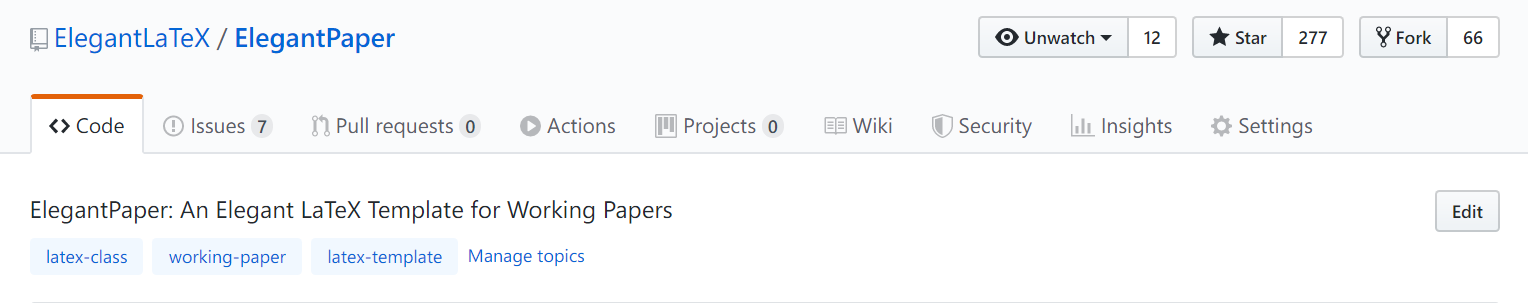
\includegraphics[width=\textwidth]{star.png}
	\caption{Twinkle, Twinkle, Little Star}
\end{figure}

\section{Donation}
To express your love for our templates and/or our developers, please do not hesitate to tip us.
\begin{figure}[!htbp]
	\centering
	
\includegraphics[width=0.4\textwidth]{donate.jpg}
\end{figure}

\textbf{The explanation right of the tip usage belongs to Elegant\LaTeX{} with no supervision. Feel free to tip us.} Those who donate more than 10 RMB will be recorded in the donation list. Thank all the tippers!


\begin{table}[!htb]
	\centering
	\caption{Donation List}
	\begin{tabular}{*{4}{>{\scriptsize}c}|*{4}{>{\scriptsize}c}}
	  \toprule
	  \textbf{Tipper} & \textbf{Amount} & \textbf{Date} & \textbf{Channel} & \textbf{Tipper} & \textbf{Amount} & \textbf{Date} & \textbf{Channel} \\
	  \midrule
	  Lerh  & 10 RMB & 2019/05/15 & Wechat    & yueguodipingxian & 10 RMB & 2019/05/15 & Wechat \\
	  yinsang    & 20 RMB & 2019/05/27 & Wechat    & *kong    & 10 RMB & 2019/05/30 & Wechat \\
	  latexstudio.net & 666 RMB & 2019/06/05 & Alipay   & A*n   & 40 RMB & 2019/06/15 & Wechat \\
	  * xia   & 22 RMB & 2019/06/15 & Wechat    & * qian  & 21 RMB  & 2019/06/15 & Wechat \\
	  Cassis & 11 RMB & 2019/06/30 & Wechat    & * jun    & 10 RMB & 2019/07/23 & Wechat \\
	  P*u   & 50 RMB & 2019/07/30 & Wechat    & * meng    & 19 RMB & 2019/08/28 & Wechat \\
	  Qu Doudou   & 10 RMB & 2019/08/28 & Wechat    & Li Bo    & 100 RMB & 2019/10/06 & Wechat \\
	  Njustsll & 10 RMB & 2019/10/11 & Wechat    & Liu Zhikuo   & 99.99 RMB & 2019/10/15 & Alipay \\
	  * tao   & 16 RMB & 2019/10/17 & Wechat    & Chini    & 12 RMB & 2019/10/17 & Alipay \\
	  yuanfengjing & 10 RMB & 2019/10/28 & Wechat    & Guo Deliang   & 88 RMB & 2019/11/03 & Wechat \\
	  ziqiangbuxi  & 20 RMB & 2019/11/04 & Alipay   & dushuzhichong  & 20 RMB & 2019/11/18 & Wechat \\
	  * deng    & 10 RMB & 2019/11/18 & Wechat    & * zhe   & 20 RMB & 2019/11/18 & Wechat \\
	  anonymous    & 10 RMB & 2019/11/24 & Wechat    & Jiye Qian & 66 RMB & 2019/12/04 & Wechat \\
	  * yang   & 20 RMB & 2019/12/05 & Wechat    & Catcher & 11 RMB & 2019/12/08 & Alipay \\
	  xierbotementu & 10 RMB & 2019/12/09 & Alipay   & * wei   & 10 RMB & 2019/12/09 & Wechat \\
	  Simon & 20 RMB & 2019/12/11 & Alipay   & liushangqianyi & 66.60 RMB & 2019/12/18 & Alipay \\
	  yu     & 10 RMB & 2019/12/20 & Alipay   & *chen   & 15 RMB & 2019/12/20 & Wechat \\
	  suifeng   & 20 RMB & 2019/12/27 & Alipay   & Ws    & 23.30 RMB & 2019/12/28 & Wechat \\
	  chuba    & 100 RMB  & 2020/01/02 & Alipay   & p*e   & 20 RMB & 2020/01/03 & Wechat \\
	  Shunmx & 100 RMB & 2020/01/03 & Wechat    & hj    & 10 RMB & 2020/01/03 & Wechat \\
	  F*5   & 10 RMB & 2020/01/03 & Wechat    & S*m   & 20.20 RMB & 2020/01/03 & Wechat \\
	  erdaiqingzhi  & 13 RMB & 2020/01/14 & Alipay   & *?    & 66 RMB & 2020/01/15 & Wechat \\
	  Mr. Xiong & 20 RMB & 2020/01/17 & Wechat    & *bo    & 15 RMB & 2020/01/18 & Wechat \\
	  *Zhe    & 10 RMB & 2020/02/02 & Wechat    &  Jackie &  88.80 RMB  &  2020/02/09 & Wechat \\
	  Henry\_Sun & 50 RMB & 2020/02/14 & Alipay & * Qiao  & 50 RMB & 2020/02/21 & Wechat \\
	  YunLian & 10 RMB & 2020/03/02 & Alipay & S*y  &  10 RMB  &  2020/03/15 & Wechat \\
	  * Ge  & 66.66 RMB & 2020/03/17 & Wechat    &   K*e & 30 RMB & 2020/03/30 & Wechat\\
	  * Yang  &  20 RMB  &  2020/04/02 & Wechat & Shi*n  & 30 RMB & 2020/04/11 & Wechat \\
	  \bottomrule
	\end{tabular}%
	\label{tab:donation}%
  \end{table}%

\section{FAQ}

\begin{enumerate}[label=\arabic*).]
	\item \textit{How to remove the information of version?}\\
    Please comment \lstinline|\version{x.xx}|.
	\item \textit{How to remove the information of date?}\\
	Please type in \lstinline|\date{}|.
	\item \textit{How to add several authors?}\\
	Use \lstinline{\and} in \lstinline{\author} and use \lstinline{\\} to start a new line.
	\begin{lstlisting}
	\author{author 1\\ org. 1 \and author 2 \\ org. 2 }
	\end{lstlisting}
	\item \textit{How to display bilingual abstracts?}\\
	Please refer to \href{https://github.com/ElegantLaTeX/ElegantPaper/issues/5}{GitHub::ElegantPaper/issues/5}
\end{enumerate}


\nocite{en1,en2}

\bibliography{wpref}

\appendix
%\appendixpage
\addappheadtotoc


\section{Use newtx fonts}
If you use \lstinline{newtx} fonts, type in:

\begin{lstlisting}
\documentclass[math=newtx]{elegantbook}
\end{lstlisting}


\subsection{Hyphens}
Since the template uses \lstinline{newtx}, please pay attention to the hyphens. For instance,
\begin{equation}
\int_{R^q} f(x,y) dy.\emph{of\kern0pt f}
\end{equation}

The corresponding code is: 
\begin{lstlisting}
\begin{equation}
\int_{R^q} f(x,y) dy.\emph{of \kern0pt f}
\end{equation}
\end{lstlisting}

\subsection{Symbol Fonts}
Feedback from ElegantBook users claims that error occurs when using our templates with  \lstinline{yhmath}, \lstinline{esvect} and other packages.
\begin{lstlisting}
LaTeX Error:
Too many symbol fonts declared.
\end{lstlisting}

The reason is that the template redefines font for math so that no new math font is allowed to be added. To use \lstinline{yhmath} and/or \lstinline{esvect}, please locate \lstinline{yhmath} or \lstinline{esvect} in \lstinline{elegantpaper.cls}, uncomment corresponding related code.

\begin{lstlisting}
%%% use yhmath pkg, uncomment following code
% \let\oldwidering\widering
% \let\widering\undefined
% \RequirePackage{yhmath}
% \let\widering\oldwidering

%%% use esvect pkg, uncomment following code
% \RequirePackage{esvect}
\end{lstlisting}

\end{document}
